\section{A second level, the containers}
\begin{frame}
Container technology is not very old \newline
\vspace{0.5cm}
The most famous: 
\includegraphics[width=0.2\textwidth]{images/docker_logo2.png} \newline
\vspace{0.5cm}
Solomon Hykes was inspirated by container port in the world travel \newline
\vspace{0.5cm}
\centering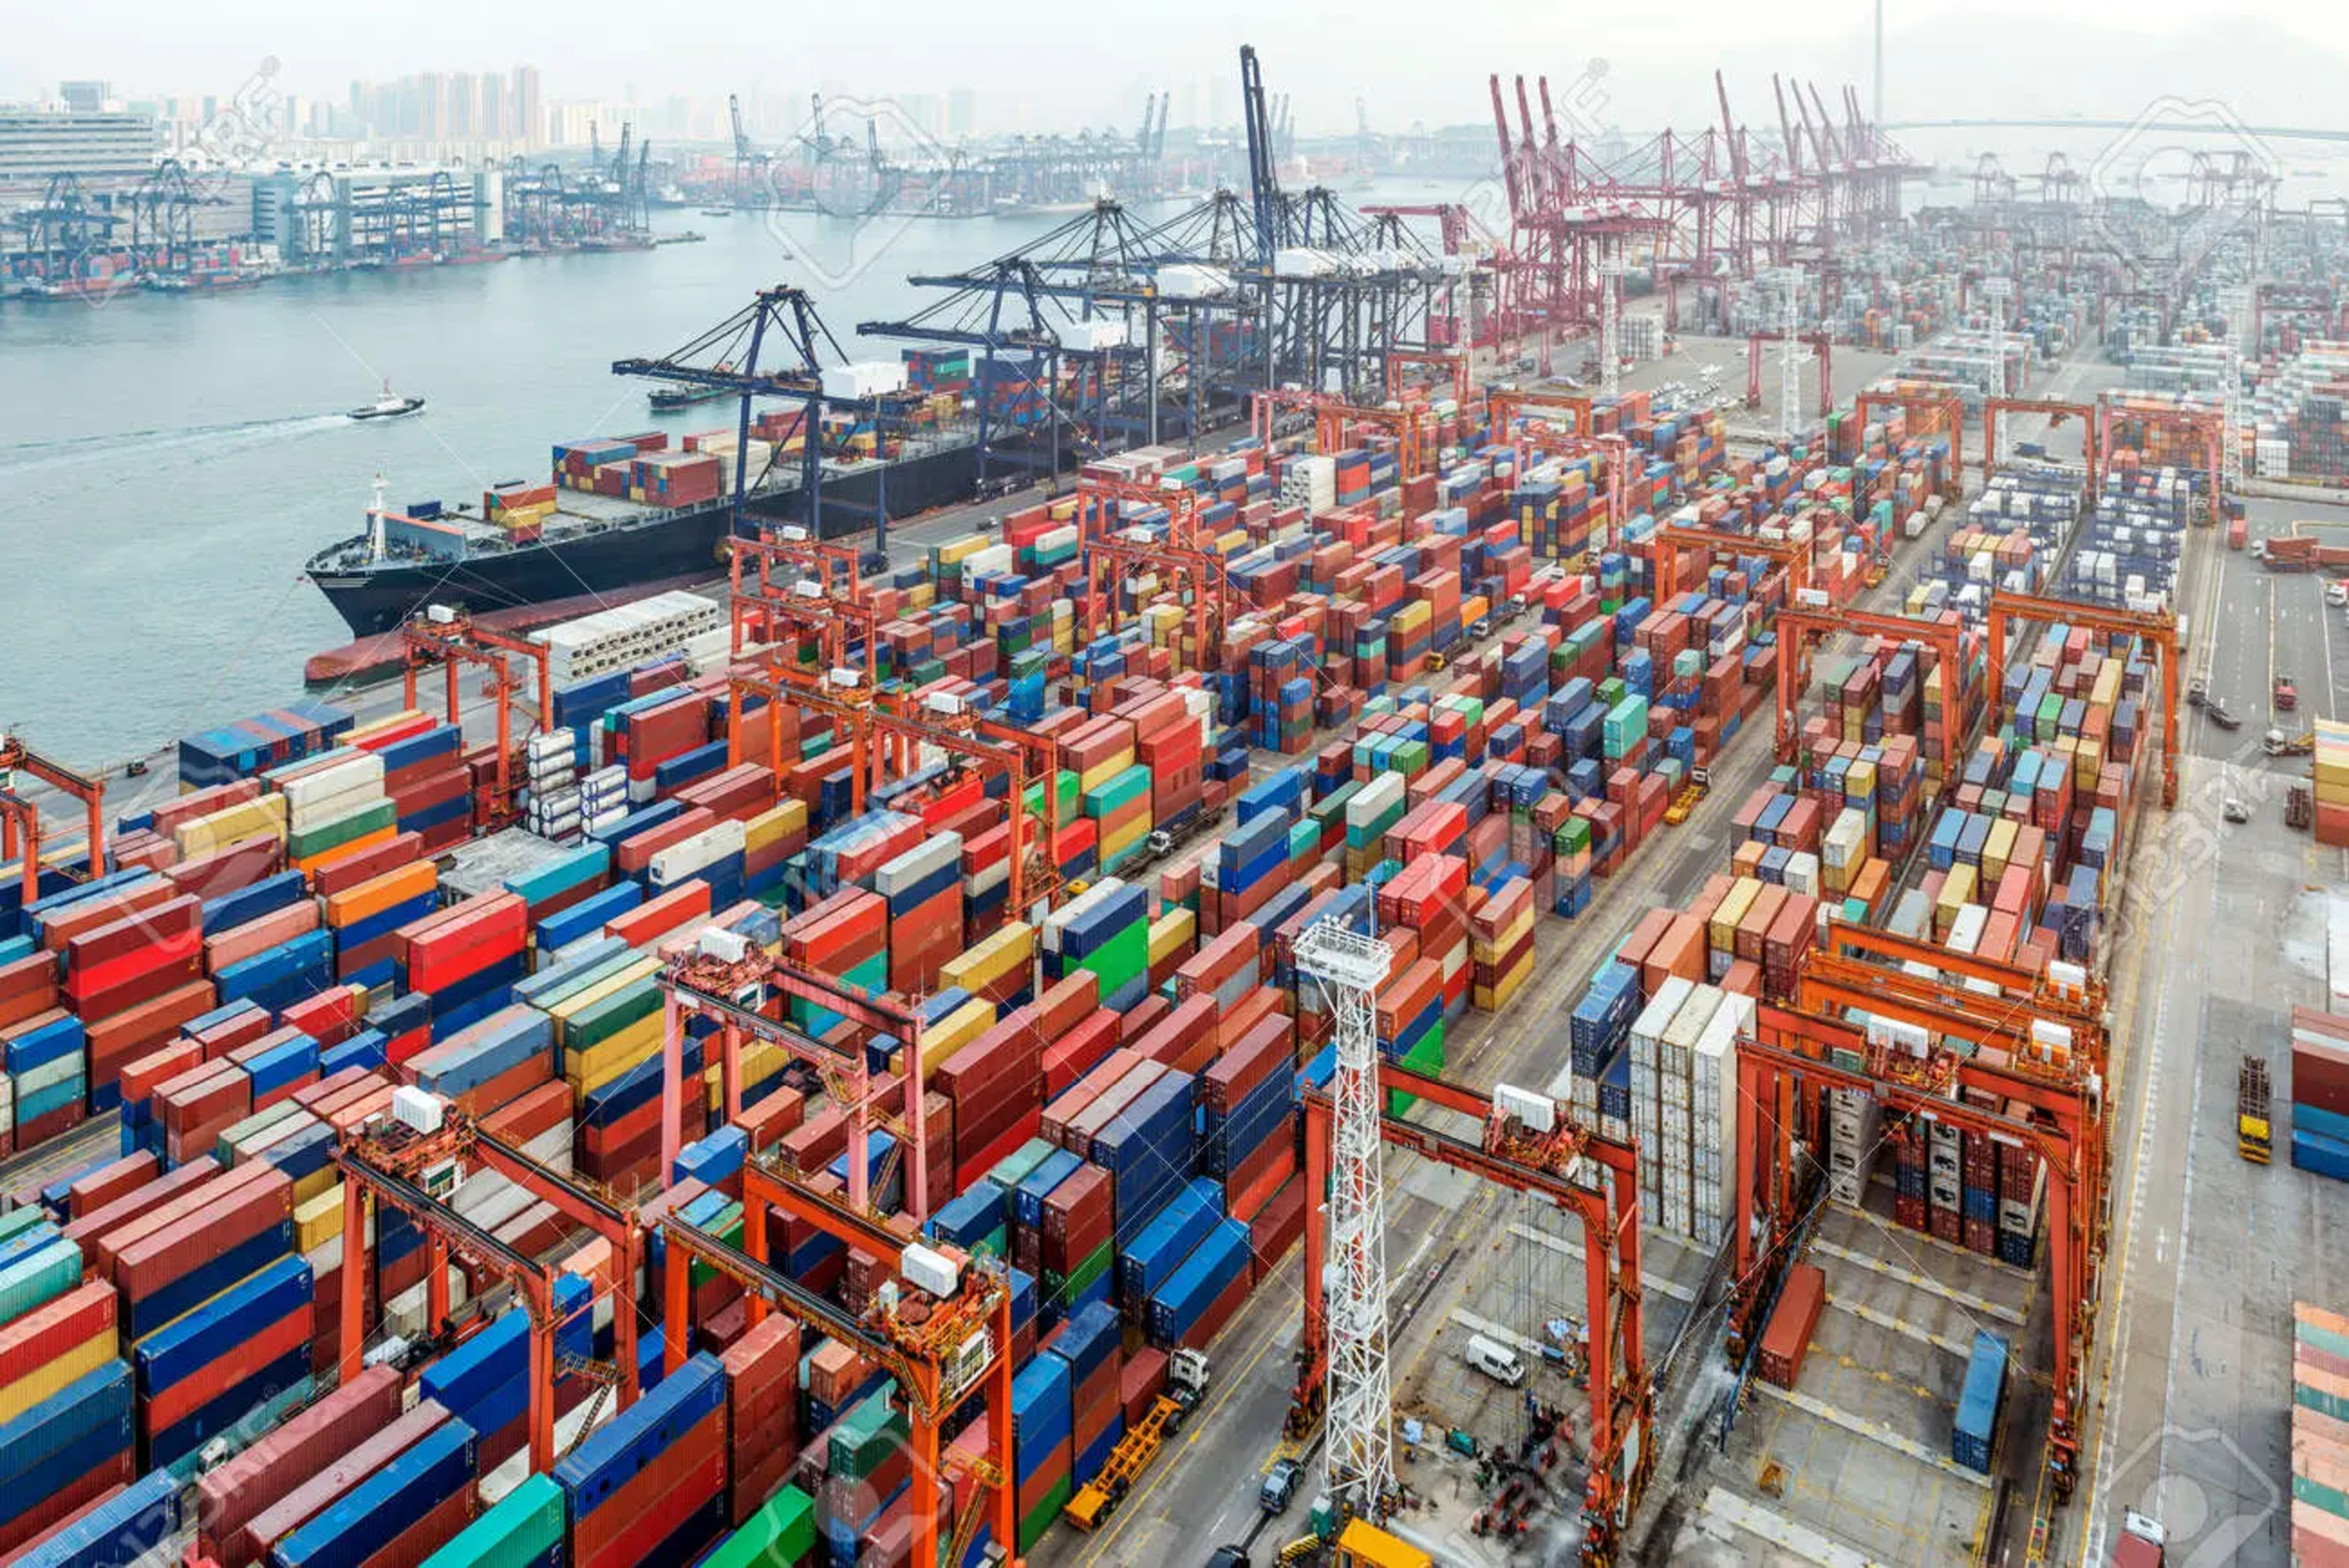
\includegraphics[width=0.4\textwidth]{images/container_port.pdf} \newline
Docker is an open source project, a community and a private company 
\end{frame}

\begin{frame}
\begin{itemize}
\item Born in 2010
\item First public release in 2013
\item V 1.0 in 2014
\item Open source and free
\item Packaged to Ubuntu in 2014 (V14.04)
\end{itemize}
\end{frame}

\subsection{Docker}{Term definitions}
\begin{frame}
\begin{columns}
\column{.48\textwidth}
\begin{itemize}
\item Docker image --> "snapshot" immutable file
	\begin{itemize}
	\item Set of libraries, functions
	\item Static state
	\item Online Store or share
	\item Automatically build
	\end{itemize}
\end{itemize}
\column{.48\textwidth}
\begin{itemize}
\item Docker container --> instance of an image
	\begin{itemize}
	\item Result of the image activation
	\item Can be modified
	\item Can be tunred into an image
	\item 1 image --> multiple containers 
	\end{itemize}
\end{itemize} 
\end{columns}
\end{frame}

\begin{frame}
\centering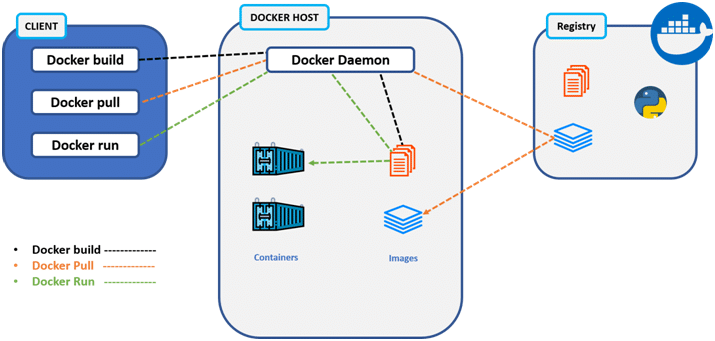
\includegraphics[width=0.7\textwidth]{images/Docker-Architecture.png}
\end{frame}
\begin{frame}[fragile]
client-server architecture
\begin{enumerate}
\item Client talk to a daemon (docker background program)
\begin{block}{Client}
\begin{verbatim}
$ docker build [path][url] 
  docker build https://github.com/docker/rootfs.git#container:docker
$ docker pull [image_name]
  docker pull biocontainers/samtools
$ docker run [image_name]
  docker run biocontainers/samtools
\end{verbatim}
\end{block}
\end{enumerate}

\end{frame}
\begin{frame}
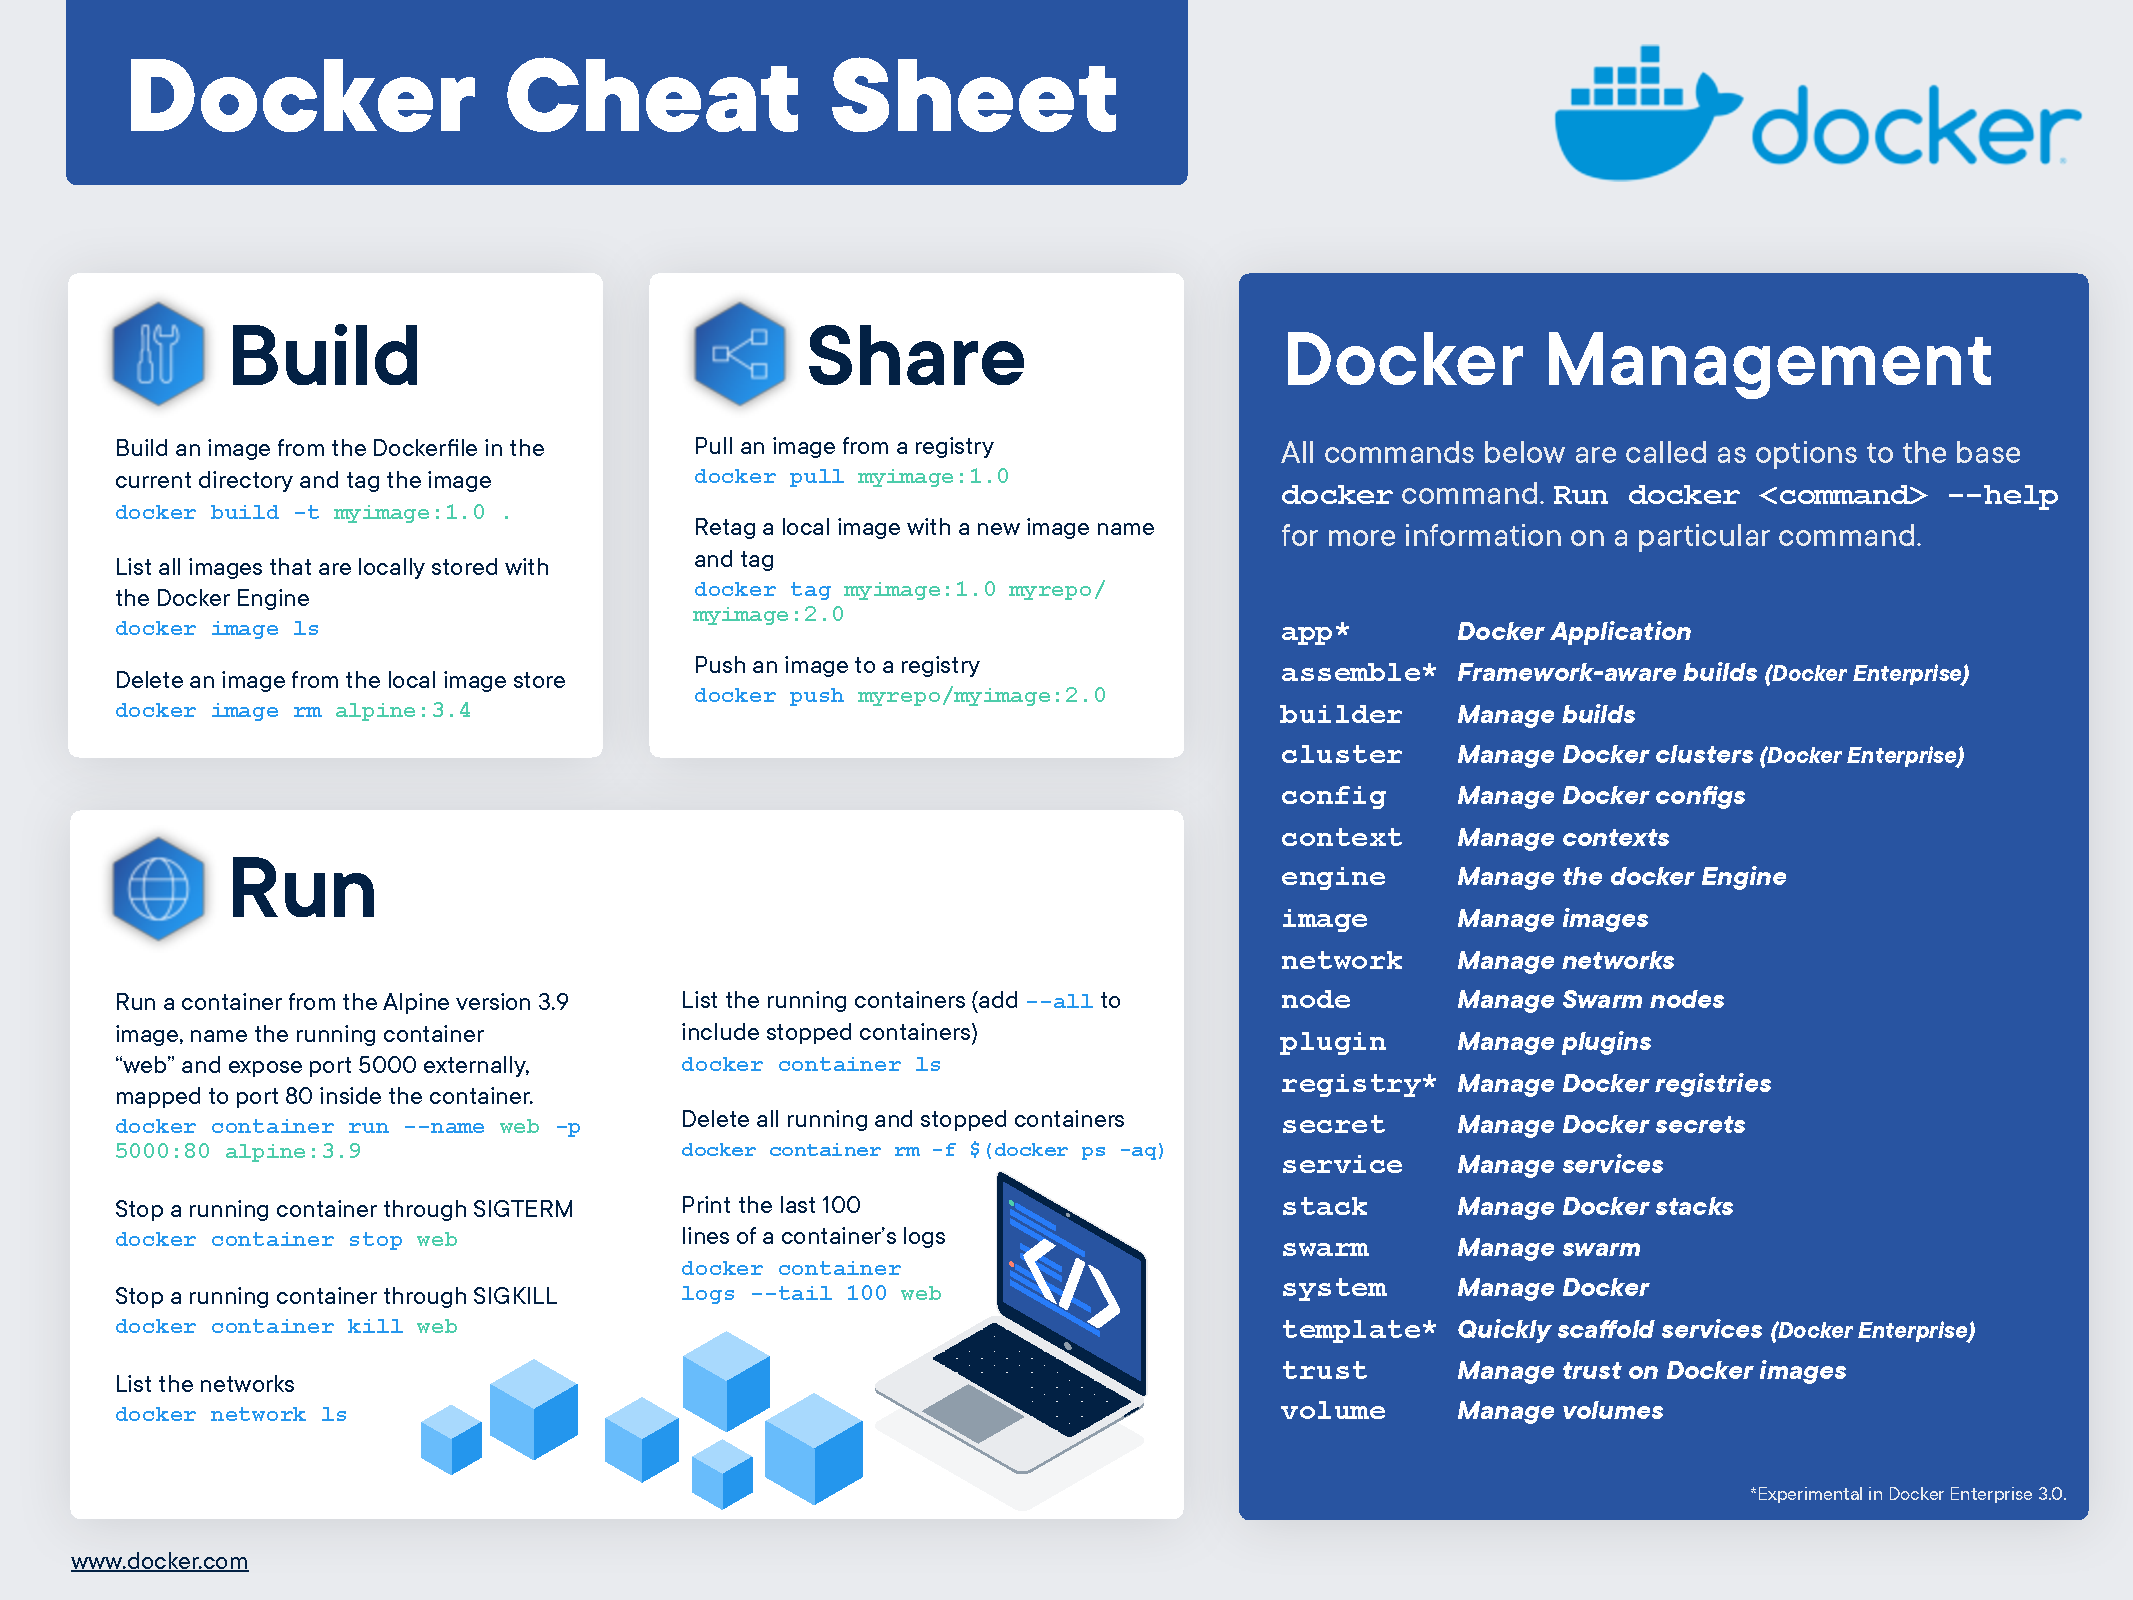
\includegraphics[width=0.45\textwidth]{images/docker-cheat-sheet.pdf}
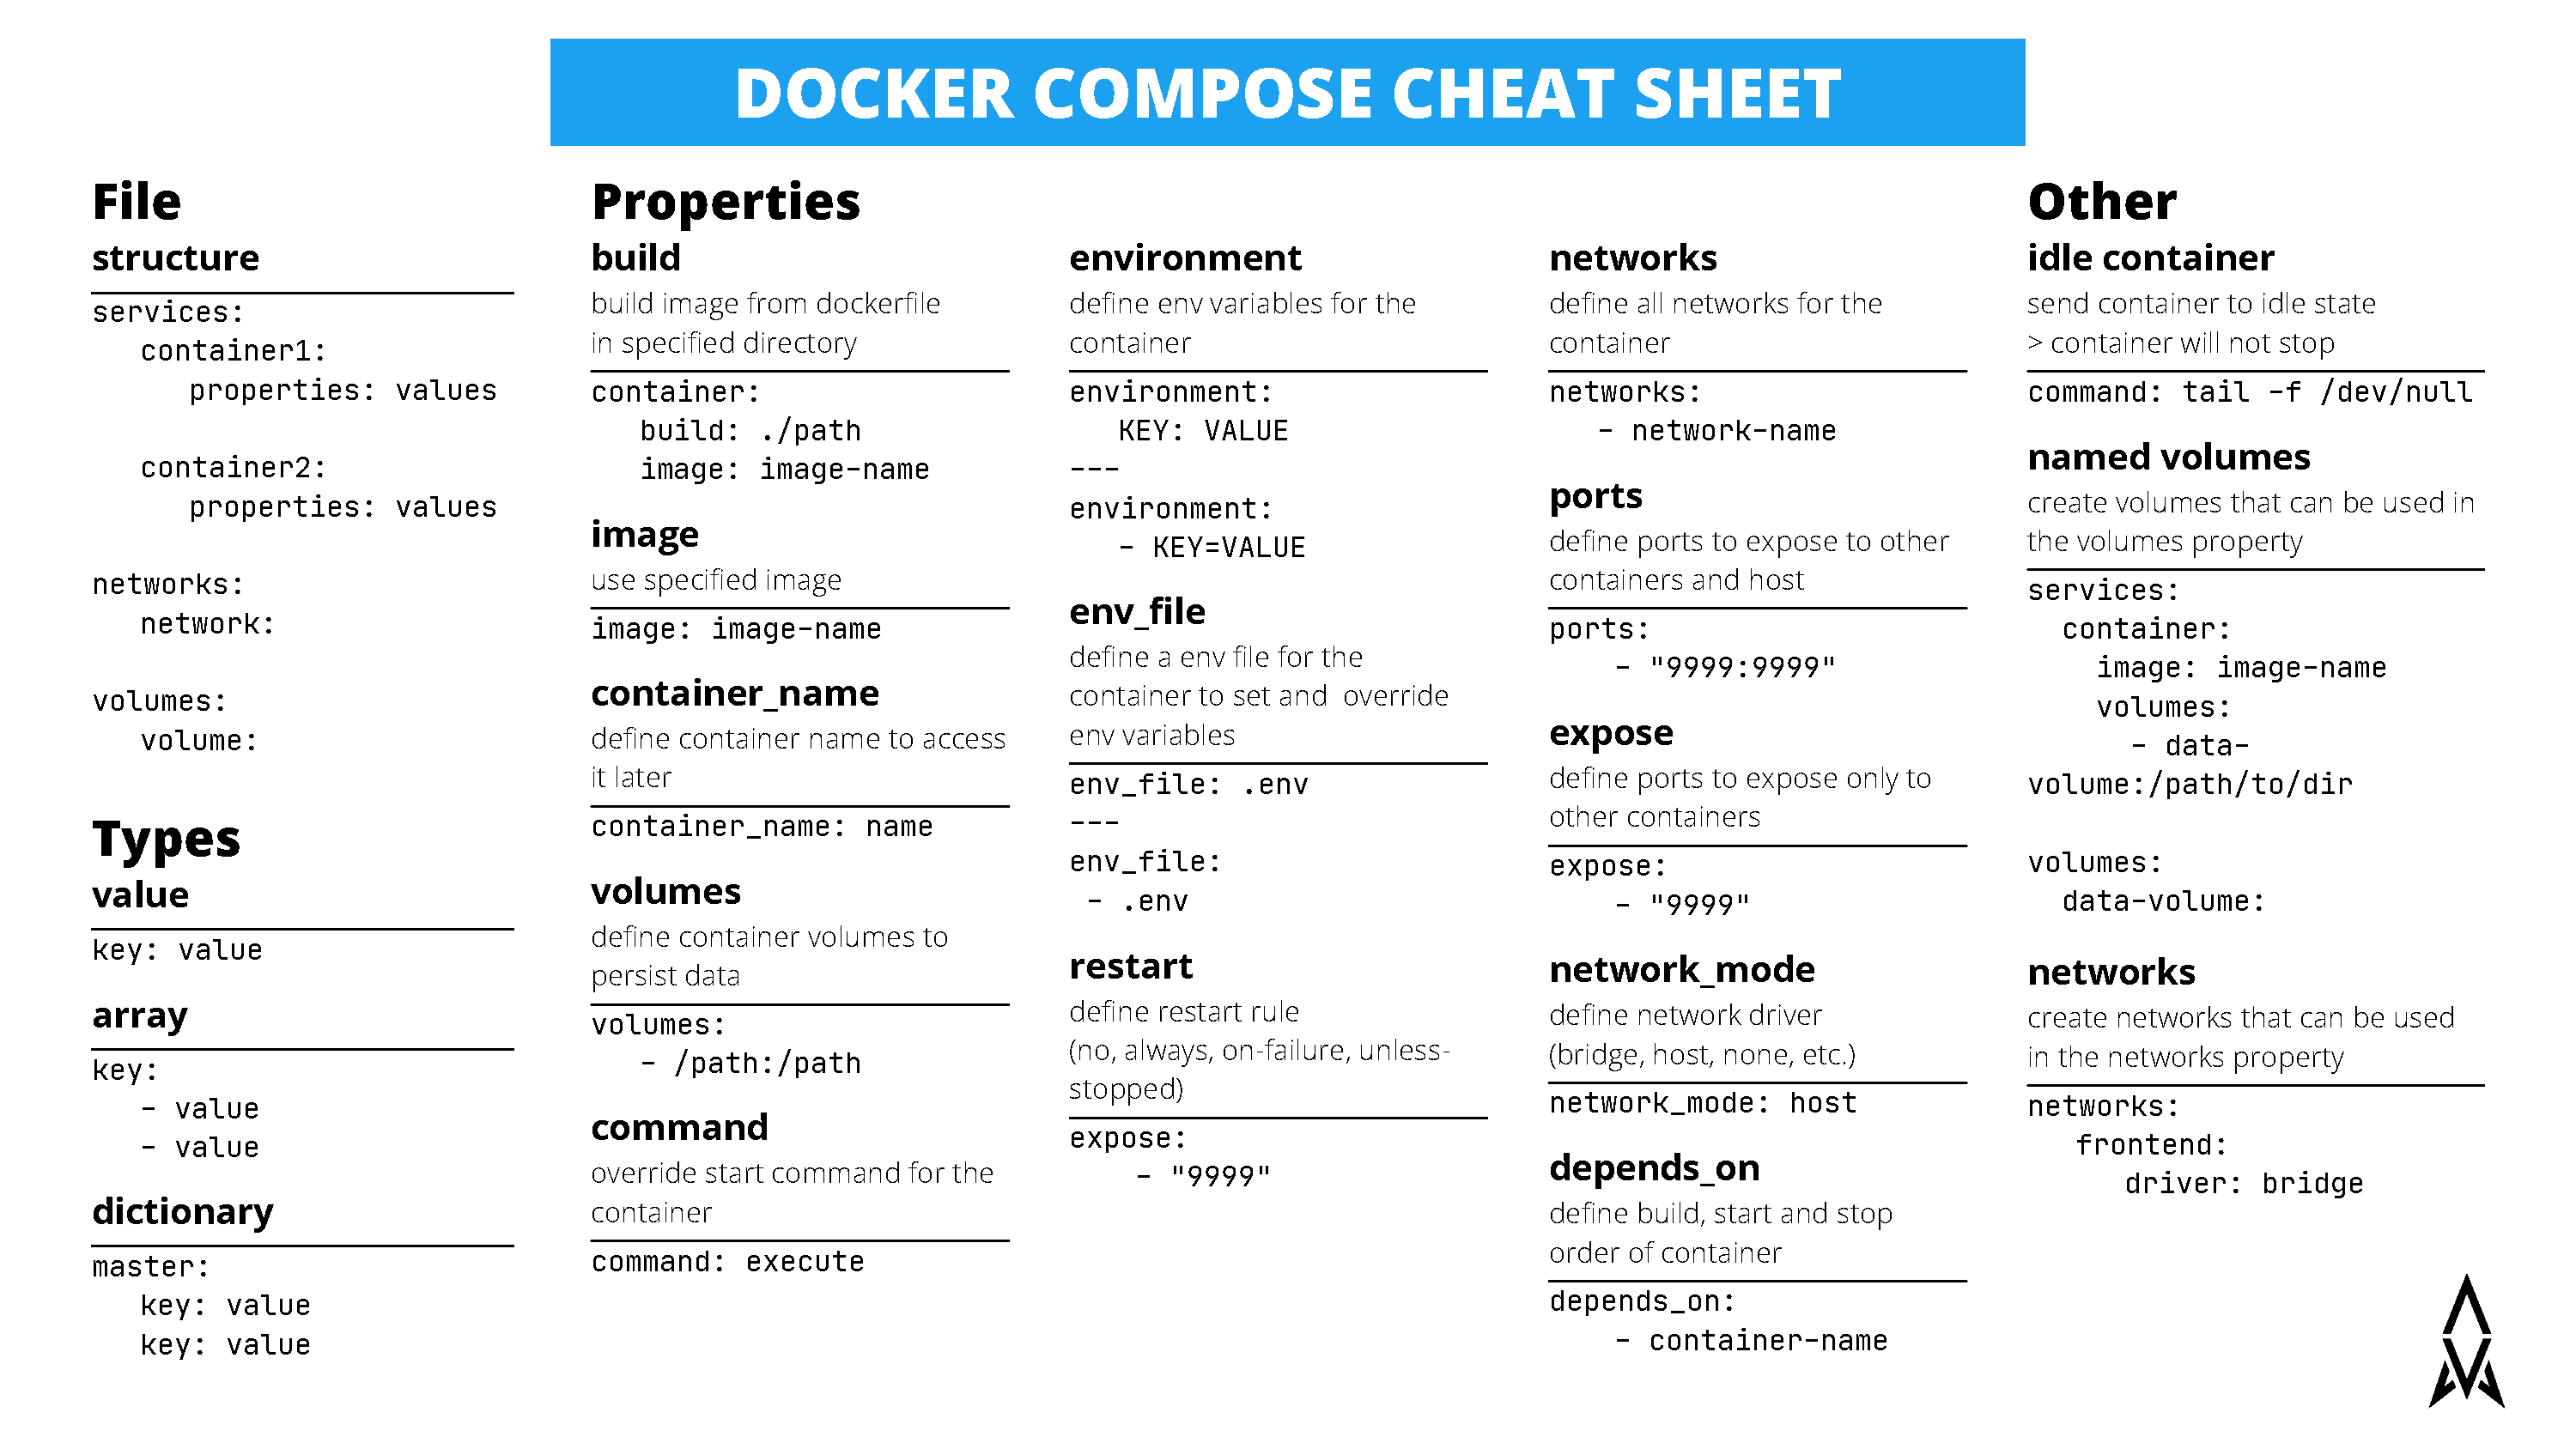
\includegraphics[width=0.45\textwidth]{images/docker-compose-cheat-sheet.pdf}

\end{frame}
\subsection{Singularity}


